%% Creator: Inkscape 0.91, www.inkscape.org
%% PDF/EPS/PS + LaTeX output extension by Johan Engelen, 2010
%% Accompanies image file 'Inverzni_filtr.pdf' (pdf, eps, ps)
%%
%% To include the image in your LaTeX document, write
%%   \input{<filename>.pdf_tex}
%%  instead of
%%   \includegraphics{<filename>.pdf}
%% To scale the image, write
%%   \def\svgwidth{<desired width>}
%%   \input{<filename>.pdf_tex}
%%  instead of
%%   \includegraphics[width=<desired width>]{<filename>.pdf}
%%
%% Images with a different path to the parent latex file can
%% be accessed with the `import' package (which may need to be
%% installed) using
%%   \usepackage{import}
%% in the preamble, and then including the image with
%%   \import{<path to file>}{<filename>.pdf_tex}
%% Alternatively, one can specify
%%   \graphicspath{{<path to file>/}}
%%
%% For more information, please see info/svg-inkscape on CTAN:
%%   http://tug.ctan.org/tex-archive/info/svg-inkscape
%%
\begingroup%
  \makeatletter%
  \providecommand\color[2][]{%
    \errmessage{(Inkscape) Color is used for the text in Inkscape, but the package 'color.sty' is not loaded}%
    \renewcommand\color[2][]{}%
  }%
  \providecommand\transparent[1]{%
    \errmessage{(Inkscape) Transparency is used (non-zero) for the text in Inkscape, but the package 'transparent.sty' is not loaded}%
    \renewcommand\transparent[1]{}%
  }%
  \providecommand\rotatebox[2]{#2}%
  \ifx\svgwidth\undefined%
    \setlength{\unitlength}{240bp}%
    \ifx\svgscale\undefined%
      \relax%
    \else%
      \setlength{\unitlength}{\unitlength * \real{\svgscale}}%
    \fi%
  \else%
    \setlength{\unitlength}{\svgwidth}%
  \fi%
  \global\let\svgwidth\undefined%
  \global\let\svgscale\undefined%
  \makeatother%
  \begin{picture}(1,0.76666667)%
    \put(0.82498468,0.59219774){\color[rgb]{0,0,0}\makebox(0,0)[lb]{\smash{\footnotesize $N(x)$}}}%
    \put(0.82498468,0.52553107){\color[rgb]{0,0,0}\makebox(0,0)[lb]{\smash{\footnotesize $H(x)$}}}%
    \put(0.82498468,0.4588644){\color[rgb]{0,0,0}\makebox(0,0)[lb]{\smash{\footnotesize $\frac{N(x)}{H(x)}$}}}%
    \put(0.45,0.57333228){\color[rgb]{0,0,0}\makebox(0,0)[rb]{\smash{\footnotesize $0.5$}}}%
    \put(0,0){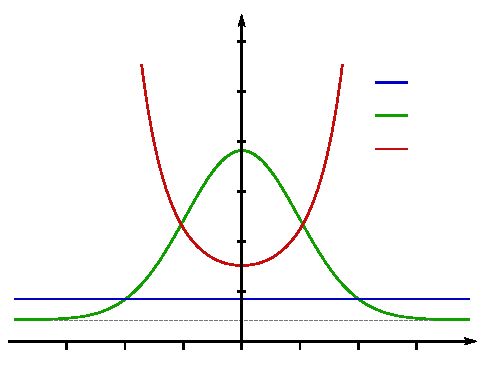
\includegraphics[width=\unitlength,page=1]{Inverzni_filtr.pdf}}%
    \put(0.48333333,0.01666562){\color[rgb]{0,0,0}\makebox(0,0)[b]{\smash{\footnotesize $0$}}}%
    \put(0.5999986,0.01666562){\color[rgb]{0,0,0}\makebox(0,0)[b]{\smash{\footnotesize $1$}}}%
    \put(0.71666527,0.01666562){\color[rgb]{0,0,0}\makebox(0,0)[b]{\smash{\footnotesize $2$}}}%
    \put(0.83333193,0.01666562){\color[rgb]{0,0,0}\makebox(0,0)[b]{\smash{\footnotesize $3$}}}%
    \put(0.13333196,0.01666562){\color[rgb]{0,0,0}\makebox(0,0)[b]{\smash{\footnotesize $-3$}}}%
    \put(0.24999723,0.01666562){\color[rgb]{0,0,0}\makebox(0,0)[b]{\smash{\footnotesize $-2$}}}%
    \put(0.3666639,0.01666562){\color[rgb]{0,0,0}\makebox(0,0)[b]{\smash{\footnotesize $-1$}}}%
    \put(0.45000118,0.67333336){\color[rgb]{0,0,0}\makebox(0,0)[rb]{\smash{\footnotesize $0.6$}}}%
    \put(0.45,0.37333336){\color[rgb]{0,0,0}\makebox(0,0)[rb]{\smash{\footnotesize $0.3$}}}%
    \put(0.45000118,0.47333447){\color[rgb]{0,0,0}\makebox(0,0)[rb]{\smash{\footnotesize $0.4$}}}%
    \put(0.45,0.17333337){\color[rgb]{0,0,0}\makebox(0,0)[rb]{\smash{\footnotesize $0.1$}}}%
    \put(0.45000118,0.27333447){\color[rgb]{0,0,0}\makebox(0,0)[rb]{\smash{\footnotesize $0.2$}}}%
  \end{picture}%
\endgroup%
